    \chapter{INTRODUCTION.}
    \lettrine[lines=2]{T}{HE arts and sciences have} become so extensive,
    that to facilitate their acquirement is of as much importance as to
    extend their boundaries. Illustration, if it does not shorten the time
    of study, will at least make it more agreeable. \textsc{This work} has
    a greater aim than mere illustration; we do not introduce colours for
    the purpose of entertainment, or to amuse \textit{by certain
    combinations of tint and form}, but to assist the mind in its
    researches after truth, to increase the facilities of instruction, and
    to diffuse permanent knowledge. If we wanted authorities to prove the
    importance and usefulness of geometry, we might quote every
    philosopher since the days of Plato. Among the Greeks, in ancient, as
    in the school of Pestalozzi and others in recent times, geometry was
    adopted as the best gymnastic of the mind. In fact, Euclid's Elements
    have become, by common consent, the basis of mathematical science all
    over the civilized globe. But this will not appear extraordinary, if
    we consider that this sublime science is not only better calculated
    than any other to call forth the spirit of inquity, to elevate the
    mind, and to strengthen the reasoning faculties, but also it forms the
    best introduction to most of the useful and important vocations of
    human life. Arithmetic, land-surveying, mensuration, engineering,
    navigation, mechanics, hydrostatics, pneumatics, optics, physical
    astronomy, \&c. are all dependent on the propositions of geometry. 

    Much however depends on the first communication of any science to a
    learner, though the best and most easy methods are seldom adopted.
    Propositions are placed before a student, who though having a
    sufficient understanding, is told just as much about them on entering
    at the very threshold of the science, as gives gives him a
    prepossession most unfavourable to his future study of this delightful
    subject; or the formalitites and paraphernalia of rigour are so
    ostentatiously put forward, as almost to hide the reality. Endless and
    perplexing repetitions, which do not confer greater exactitude on the
    reasoning, render the demonstrations involved and obscure, and conceal
    from the view of the student the consecution of evidence.'' Thus an
    aversion is created in the mind of the pupil, and a subject so
    calculated to improve the reasoning powers, and give the habit of
    close thinking, is degraded by a dry and rigid memory, To raise the
    curiosity, and to awaken the listless and dormant powers of younger
    minds should be the aim of every teacher; but where examples of
    excellence are wanting, the attempts to attain it are but few, while
    eminence excites attention and produces imitation. The object of this
    Work is to introduce a method of teaching geometry, which has been
    much approved of by many scientific men in this country, as well as
    in France and America. The plan here adopted forcibly appeals to the
    eye, the most sensitive and the most comprehensive of our external
    organs, and its pre-eminence to imprint it subject on the mind is
    supported by the incontrovertible maxim expressed in the well known
    words of Horace:- 
    \begin{quotation}
        \noindent\textit{Segnius irritant animos demissa per aurem \\
        Qu\`am qu\ae sunt oculis subjecta fidelibus} \\
        A feebler impress through the ear is made,\\
        Than what is by the faithful eye conveyed.
    \end{quotation}
    All language consists of representative signs, and those sins are the
    best which effect their purposes with the greatest precision and
    dispatch. Such for all common purposes are the audible signs called
    words, which are still considered as audible, whether addressed
    immediately to the ear, or through the medium of letteers to the ete.
    Geomerical science, the object of which is to show th erelative
    quantities of their parts by a process of reasoning called
    Demonstration. This reasoning has been generally carried on by words,
    letters, and black or uuncoloured diagrams; but as the use of coloured
    symbols, signs and diagrams in the linear arts and sciences, renders
    the process of reasoning more precise, and the attainment more
    expeditious, they have been in this instance accordingly adopted. 

    Such is the expedition of this enticing mode of communicating
    knowledge, that the Elements of Euclid can be acquired in less than
    one third the time usually emploted, and the retention by the memory
    is much more permanent; these facts have been ascertained by numerious
    experiments made by the invenror, and seveeral orhers who have adopted
    his plans. The particularsof which are few and obvious; the letters
    annexed to points, lines, or other parts of a diagram are in fact but
    arbitrary names, and represent them in the demonstration; instead of
    these, the parts being differently colouresd, are made to name
    themselves, for their forms in corresponding colours represent them in
    the demonstration. 

    In order to give a better idea of this system, and of the advantages
    gained by its adoption, let us take a right angled triangle, and
    express some of its properties both by colours and the method
    generally employed. 
    \newcommand{\cab}{
        
\begin{tikzpicture}[scale=2]
            \path[fill=red] (0,0) ++ (0.5,0) arc (0:36:0.5) -- (0,0);
        \end{tikzpicture}
    }
    \newcommand{\abc}{
        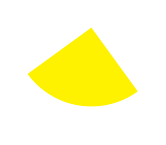
\begin{tikzpicture}[baseline=-6.0ex,rotate=216,scale=2]
            \path[fill=yellow] (0,0) ++ (0.5,0) arc (0:90:0.5) -- (0,0);
        \end{tikzpicture}
    }
    \newcommand{\bca}{
        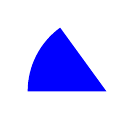
\begin{tikzpicture}[rotate=126,scale=2]
            \path[fill=blue] (0,0) ++ (0.5,0) arc (0:54:0.5) -- (0,0);
        \end{tikzpicture}
    }

    \begin{figure}
    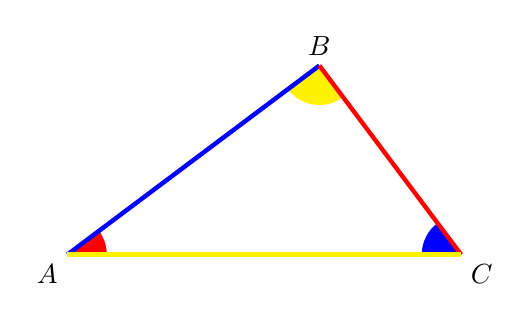
\begin{tikzpicture}
        \coordinate (A) at (0,0);
        \coordinate (B) at (3.2,2.4);
        \coordinate (C) at (5,0);
        \path[fill=red,ultra thick] (A) ++(0.5,0) arc (0:36:0.5) -- (A);
        \path[fill=yellow,ultra thick] (B) ++(-90+36:0.5) arc (-90+36:-180+36:0.5) -- (B);
        \path[fill=blue,ultra thick] (C) ++(-0.5,0) arc (180:90+36:0.5) -- (C);
        \node[below left ] at (A) {$A$};
        \node[above      ] at (B) {$B$};
        \node[below right] at (C) {$C$};
        \draw[blue,ultra thick]   (A) -- (B);
        \draw[red,ultra thick]    (B) -- (C);
        \draw[yellow,ultra thick] (C) -- (A);
    \end{tikzpicture}
    \end{figure}

    \begin{center}
        \textit{Some of the properties of the right angled triangle 
        \textrm{ABC}, expressed by the method generally employed.}
    \end{center}

    \begin{enumerate}
        \item The angle BAC, together with the angles BCA and ABC are 
            equal to two right angles, or twice the angle ABC. 
        \item The angle CAB added to the angle ACB will be equal to 
            the angle ABC. 
        \item The angle ABC is greater than either of the 
            angles BAC or BCA. 
        \item The angle BCA or the angle CAB is less than the 
            angle ABC. 
        \item If from the angle ABC, there be taken the angle BAC, 
            the remainder will be equal to the angle ACB. 
        \item The square of AC is equal to the sum of the squares 
            of AB and BC. 
    \end{enumerate}

    \begin{center}
        \textit{The same properties expressed by colouring 
        the different parts.}
    \end{center}

    \begin{enumerate}
        \item \[ \cab \plus \abc \plus \bca \equals 2\, \abc \equals \rightangles.\]
          That is, the red angle added to the yellow angle added to the blue angle, equal twice the yellow angle, equal two right angles. 
      \item \[\cab \plus \bca \equals \abc.\] 
          Or in words, the red angle added to the blue angle, equal the yellow angle. 
      \item \[\abc \greater \cab \text{ or } \greater \bca.\]
          The yellow angle is greater than either the red of blue angle. 
      \item \[\cab \text{ or } \bca \less\abc.\]
          Either the red or blue angle is less than the yellow angle.
      \item \[\abc \text{ minus } \bca \equals \cab.\]
          In other terms, the yellow angle made less by the blue angle equal the red angle. 
      \item \[\tikzhline[yellow]{1.2cm}^{2} \equals \tikzhline[blue]{1.2cm}^{2} \plus \tikzhline[red]{1.2cm}^{2}.\]
          That is, the square of the yellow line is equal to the sum of the squares of the blue and red lines. 
    \end{enumerate}

    In oral demonstrations we gain with colours this important advantage, the 
    eye and the ear can be addressed at the same moment, so that for teavhing 
    geometry, and other linear arts and sciences, in classes, the ststem is 
    the best ever proposed, this is apparent from the examples just 
    given. 

    Whence it is evident that a reference from the text to the diagram is more 
    rapid and sure, by giving the forms and colours of the parts, or by 
    naming the parts and their colours, than naming the parts and letters on 
    the diagram. Besides the superior simplicity, this system is likewise 
    conspicuous for concentration, and wholly excludes the injrious though 
    prevalent practice of allowing the student to commit the demonstration 
    to memory; until reason , and fact, and proof only make impressions on 
    the understanding. 

    Again, when lecturing on the principles or properties of figures, if we 
    mention the colour of the part or parts referred to, as in saying, the 
    red angle, the blue line, or lines, \&c.~the part or parts thus names 
    will be immediately seen by all in the class at the same instant; not so 
    if we say the angle ABC, the triangle PFQ, the figure EGKt, and so on; 
    for the letters must be traces one by one before the students arrange in 
    their minds the particular magnitude reeferred to, which often occasions 
    confusino and error, as well as lots of time. Also if the parts which are 
    given as equal, have the same colours in any diagram, the mind will not 
    wander from the object before it; that is, such an arrangement presents 
    an ocular demonstration of the parts to be proved equal, and the learner 
    retains the data throughout the whole of the reasoning. But whatever may 
    be the advantages of the present plan, if it be not substituted for, it 
    can always be made a powerful auxiliary to the other methods, for the 
    purpose of introduction, or of a more speedt reminiscence, or of more 
    permanent retention by the memory. 

    The experience of all who have formed systems to impress facts on the 
    understanding, agree in proving that coloured representations, as 
    pictures, cuts, diagrams, \&c.~are more easily fixed in the mind than 
    mere sentences unmarked by any peculiarity. Curious as it may appear, 
    poets seem to be aware of this fact more than mathematicians; many modern 
    poets allude to this visible system of communicating knowledge, one of 
    them has thus expressed himself: 
    \begin{quotation}
        Sounds which address the ear are lost and die\\
        In one short hour, but these which strike the eye,\\
        Live long upon the mind, the faithful sight\\
        Engraves the knowledge with a beam of light.
    \end{quotation}
    This perhaps may be reckoned the only improvement on which plain 
    geometry has recerived since the dats of Euclid, and if there were any 
    geometers of note before that time, Eclid's success has quite ecliped 
    their memory, and even occasioned all good things of that kindto be 
    assigned to him; like \AE sop among the writers of Fables. It may also be 
    worthy of remark, as tangible diagrams afford only the medium through 
    which geometry and other linear arts and scoences can be taught to the 
    blind, this visible system is no less adapted to the exigencies of the 
    deaf and dumb. 

    Care must be taken to show that colour has nothing to do with the lines, angles, or magnitudes except merely to name them. A mathematical line, which is length without breadth, cannot possess colour, yet the junction of two colours on the same plane gives a good idea of what is meant by a mathematical linel recorllect we are speaking familiarly, such a junction is to be understood and not the colour,l when we say the black line, the red line or line, \&c. 

    Colours and coloured diagrams may at first appear a climsy method to convery proper notions of the properties and parts of mathematical figures and magnitudes, however they will be found to afford a means more refined and extensive than any that has been hitherto proposed. 

    We shall here define a point, a line, and a sufrace, and demonstrate a proposition in order to show the truth of this assertion. 

    A spoint is that which has position, but not magnitude; or a point is position only, abstracted from the consideration of length, breadth, and thickness. Perhaps the following descriptiobn is better calculated to explain the nature of a mathematical point to those who have no acquired the idea, than the above specious definition. 

    Let three colours meet and cover a portion of the paper, where the meet is not blue, not is it yellow, not is it red, as it occupes no potion of the plane, for it it did, it would belong to the blue, the red or the yellow part; yet it exists, and has position without magnitude, so that with a little reflection , this junction of three colours on a plane, gives a good idea of a methamtical point. 
%   DIAGRAM OF A CIRCLE HERE
    A line is length withou breadth. With the assistance of colours, nearly inthe same manner as before, and idea of a line may be thus give:--

    Let two colours meet and cover a potion of the paper; where the meet is not red, nor is it blue; therefore it cannot have breadth, but only length: from which we can readily form an idea of what is meant by a mathematical line. For the purpose of illustration, one colour differing from the colour of the paper, or plane upon which it is drawn, would have been sufficient; hence in future, if we say the red line, the blue line, or line, \& c. it is the junctions with the plane upon which they are drawn are to be understood. 
%   DIAGRAM OF A PLANE HERE
    Surface is that which has length and breadth without thickness. 

    When we consider a solid body (PQ), we perceive at once that it has three dimensions, namely:-- length, breadth, and thickness; suppose one part of this solid (PS) to be red, and the other part (QR) yellow, and that the colours be distinct without commingling, the blue surface (RS) which separates these parts, or this is the same thing, that which divides the solid without loss of material, must be without thickness, and only possesses length and breadthl this plainly appears from reasoning, similar to that just employed in defining, or rather describing a point and a line. 
% Diagram of a cuboid here
    The proposition which we have selected to elucidate the manner in which the principles are applied, is the fifth proposition of the first Book. 
%COPY THE FIFTH PROPOSITION. 







    Our object in this place being to introduce the system rather than to teach any particular set of propositions, we have therefore selected the foregoing out of the regular course. For schools and other public places of instruction, dyed chalks will answer to describe diagrams, \&c. fo rprivate use coloured pencils will be found very convenient.
    We are happy to find that the Elements of Mathematics now forms a considerable part of ever found female education, therefore we call the attention of those interested or engaged in the education of ladies to this very attractive mode of communicating knowledge, and to the successing work for its future developement. 

    We shall for the present conclude by obsercing, as the sensed of sight and hearing can be so forcibly and instantaneously addressed alike with one thousand as with one, \textit{the million} might be taught geometry and other branches of mathematics with great ease, this would advance the purpose of education more than any thing that \textit{might} be names, for it would teach the people how to think, and not what to think; it is in this particular the great error of education originates.



 
